\section{\texorpdfstring{Hazardy}{Hazardy}}

% =====================================================================================================================
	\begin{frame}
    \frametitle{Reálné vlastnosti logických IO}
	
		\begin{center}
			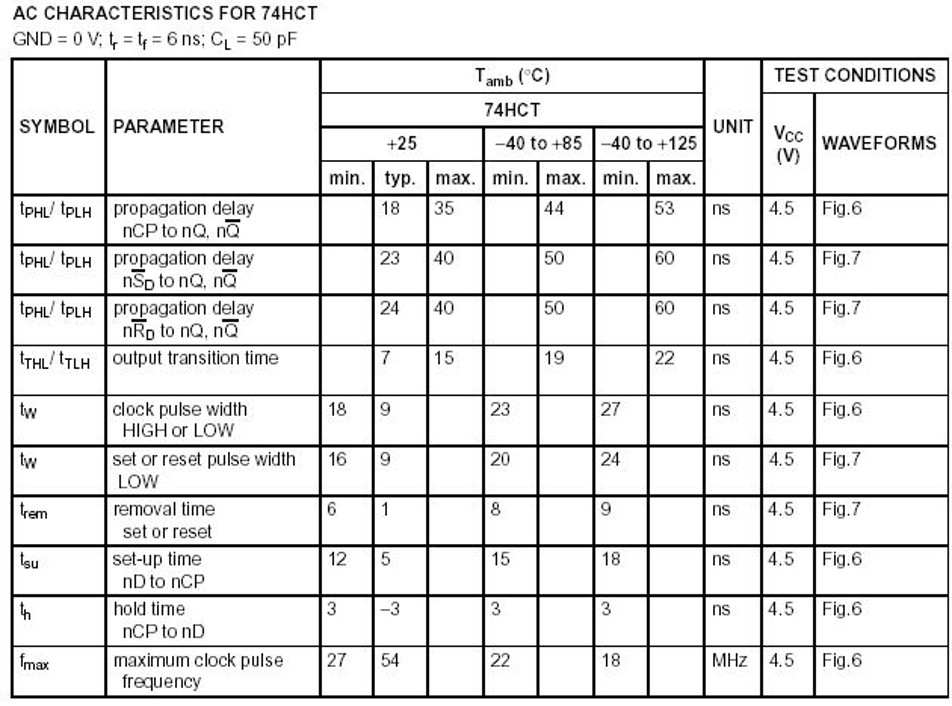
\includegraphics[width=1.00\textheight]{fig/74HCT_delays.jpg}
		\end{center}
	
	\end{frame}
	
% =====================================================================================================================
	\begin{frame}
    \frametitle{Reálné vlastnosti logických IO - D KO}
	
		\begin{center}
			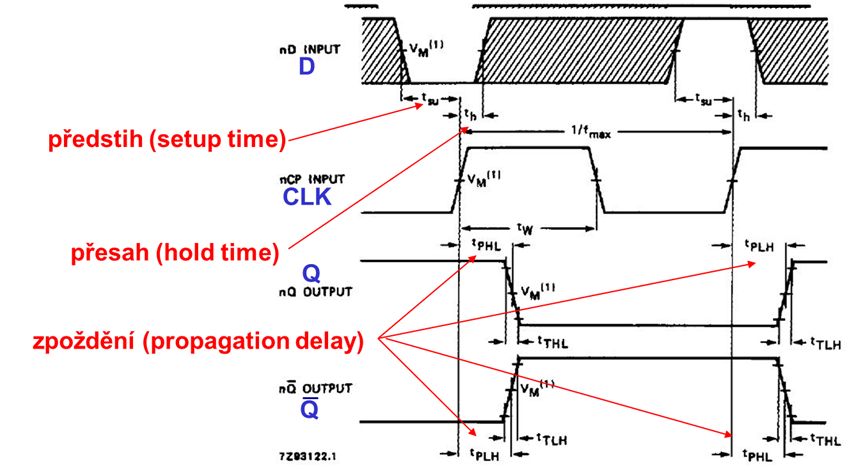
\includegraphics[width=0.95\textwidth]{fig/D_FF_delays.png}
		\end{center}
	
	\end{frame}

% =====================================================================================================================
	\begin{frame}
    \frametitle{Hazard - definice}
	
		Jde o nežádoucí přechodný děj, kdy výstup dočasně neodpovídá nastavené kombinaci vstupů.
		
		\begin{description}
		\item[\textbf{Statický}] Přechod mezi shodnými stavy (oba v log. 1 nebo 0) logické funkce způsobí krátkodobou změnu výstupu na opačný stav.
		\item[\textbf{Dynamický}] Přechod mezi stavy logické funkce způsobí několikanásobnou změnu výstupu.
		\end{description}
		
		\vspace{5mm}
		
		Hazardy obvykle dělíme na dva druhy podle toho, zda:
		
		\begin{enumerate}
			\item vzniká při změně jedné proměnné (sousední pozice v Karnaughově mapě), nebo
			\item při současné změně více proměnných.
		\end{enumerate}
	
	\end{frame}

% =====================================================================================================================
	\begin{frame}
    \frametitle{Statický hazard 1. druhu}
		
		\begin{minipage}[t][0.01\textheight][t]{0.55\textwidth}
			\tiny
			\begin{center}
				\begin{karnaugh-map}[4][2][1][$B$][$C$][$A$]
					\minterms{2,3,5,7}
					\implicant{3}{2}
					\implicant{5}{7}
					
					% ====== vlastní čáry ======

					% A = 1 (druhý řádek)
					\draw[very thick] (-0.15,1) -- (-0.15,0);

					% B = 1 (sloupce 3 a 4)
					\draw[very thick] (2,2.3) -- (4,2.3);

					% C = 1 (sloupce 2 a 3)
					\draw[very thick] (1,2.15) -- (3,2.15);

				\end{karnaugh-map}
			\end{center}
		\end{minipage}
		\begin{minipage}[t][0.01\textheight][t]{0.4\textwidth}
		
		$Y= \textcolor{red}{\bar{A}C} + \textcolor{green}{AB}$
		
		\end{minipage}
		
		\begin{minipage}[b][0.45\textheight][t]{\textwidth}
			\begin{center}
				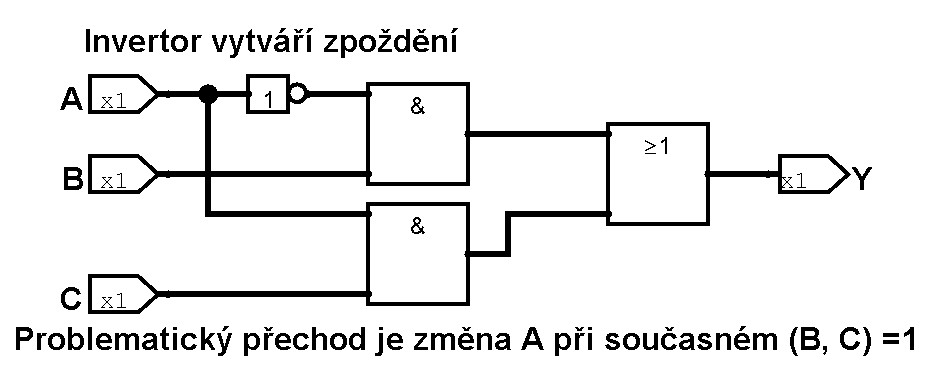
\includegraphics[scale=0.25]{fig/hazard_static.png}
			\end{center}
		\end{minipage}

	\end{frame}
	
% =====================================================================================================================
	\begin{frame}
    \frametitle{Statický hazard 1. druhu - časový diagram}
		\small
		\begin{minipage}[t][\textheight][t]{0.45\textwidth}
		\textbf{Signály:}
			\begin{center}
				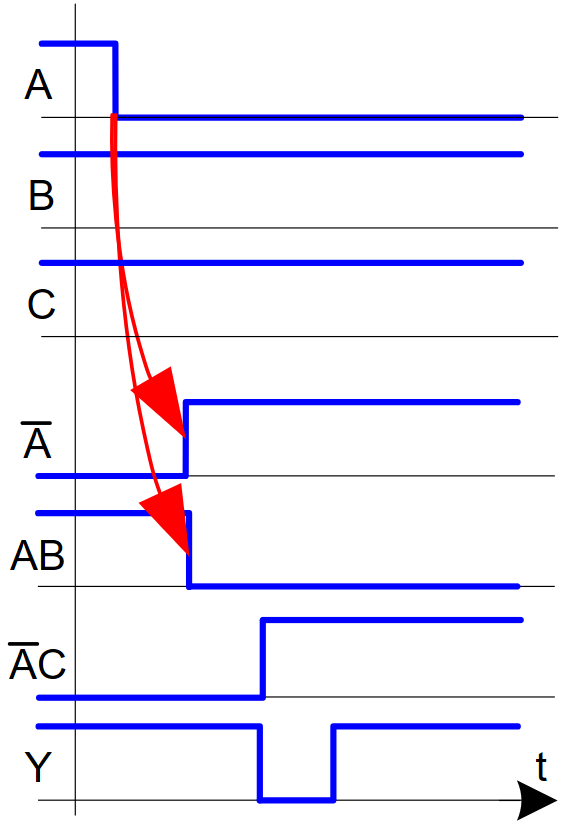
\includegraphics[width=0.85\textwidth]{fig/hazard_static_diag.png}
			\end{center}
		\end{minipage}
		\begin{minipage}[t][\textheight][t]{0.5\textwidth}
		
		Předpokládámé stejná zpoždění $t_d$ na všech hradlech:
		
		\begin{enumerate}
			\item Signál $\bar{A}$ je zpožděn za signálem $A$ o $t_d$,
			\item stejné zpoždění má i signál $AB$ a ten tlačí stav výstupu $Y$ do logické 0,
			\item logická úroveň $\bar{A}C = 1$ je vyhodnocena se zpožděním $2\times t_d$,
			\item výstup Y se vrátí do logické 1 až po příchodu hodnoty $\bar{A}C = 1$, tj. na výstupu je dočasně generována nízká úroveň po dobu zpoždění $t_d$.
		\end{enumerate}
		
		\end{minipage}

	\end{frame}
	
% =====================================================================================================================
	\begin{frame}
    \frametitle{Statický hazard 1. druhu - redundance}
		
		\begin{minipage}[t][0.01\textheight][t]{0.55\textwidth}
			\tiny
			\begin{center}
				\begin{karnaugh-map}[4][2][1][$B$][$C$][$A$]
					\minterms{2,3,5,7}
					\implicant{3}{2}
					\implicant{5}{7}
					\implicant{3}{7}
					
					% ====== vlastní čáry ======

					% A = 1 (druhý řádek)
					\draw[very thick] (-0.15,1) -- (-0.15,0);

					% B = 1 (sloupce 3 a 4)
					\draw[very thick] (2,2.3) -- (4,2.3);

					% C = 1 (sloupce 2 a 3)
					\draw[very thick] (1,2.15) -- (3,2.15);

				\end{karnaugh-map}
			\end{center}
		\end{minipage}
		\begin{minipage}[t][0.01\textheight][t]{0.4\textwidth}
		
		$Y= \textcolor{red}{\bar{A}C} + \textcolor{green}{AB} + \textcolor{orange}{BC}$
		
		\end{minipage}
		
		\begin{minipage}[b][0.45\textheight][t]{\textwidth}
			\begin{center}
				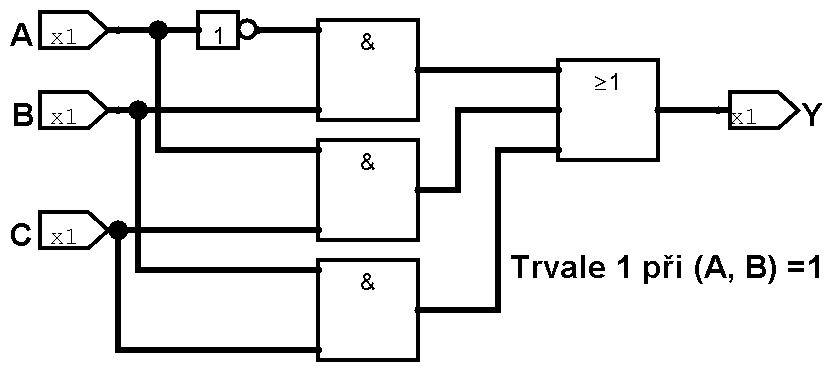
\includegraphics[scale=0.25]{fig/hazard_static_solution.png}
			\end{center}
		\end{minipage}

	\end{frame}
	
% =====================================================================================================================
	\begin{frame}
    \frametitle{Rozdíly mezi asynchronním a synchronním čítačem}
		\small
		\begin{minipage}[t][\textheight][t]{0.48\textwidth}
		
		
			\textbf{Asynchronní čítač}
			
			\vspace{3mm}
			\begin{center}
				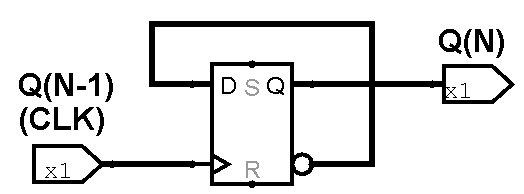
\includegraphics[scale=0.2]{fig/CU_asynch.png}
			\end{center}
			
			\vspace{5mm}
			\begin{itemize}
				\item[\textcolor{green}{\textbf{+}}] Obsahuje jen jeden typ hradla (KO),
				\item[\textcolor{green}{\textbf{+}}] velmi jednoduchá realizace,
				\item[\textcolor{red}{\textbf{-{}-{}-}}] výstupy mají vzájemné zpoždění, navazující obvody mohou vykazovat hazardy.
			\end{itemize}
			
		\end{minipage}
		\begin{minipage}[t][\textheight][t]{0.48\textwidth}
		
			\textbf{Synchronní čítač}
			
			\begin{center}
				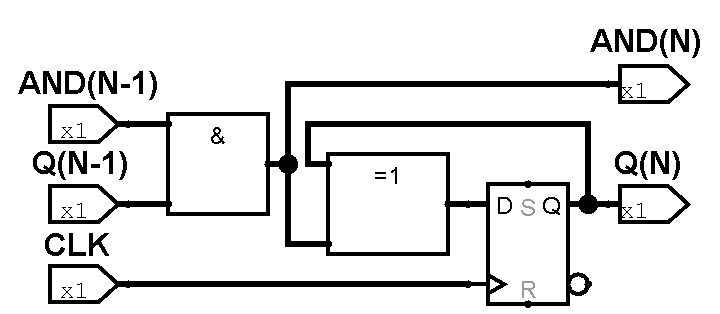
\includegraphics[scale=0.2]{fig/CU_synch.png}
			\end{center}
			
			\begin{itemize}
				\item[\textcolor{red}{\textbf{-}}] Obsahuje nejméně dva typy hradel (JK KO + AND),
				\item[\textcolor{red}{\textbf{-}}] složitější realizace,
				\item[\textcolor{green}{\textbf{+++}}] všechny výstupy se změní v jeden okamžik hrany \textbf{CLK}.
			\end{itemize}
		
		\end{minipage}

	\end{frame}
	
% =====================================================================================================================
	\begin{frame}
    \frametitle{Statický hazard 1. druhu - synchronizace}
		\small
		
		
		\begin{center}
			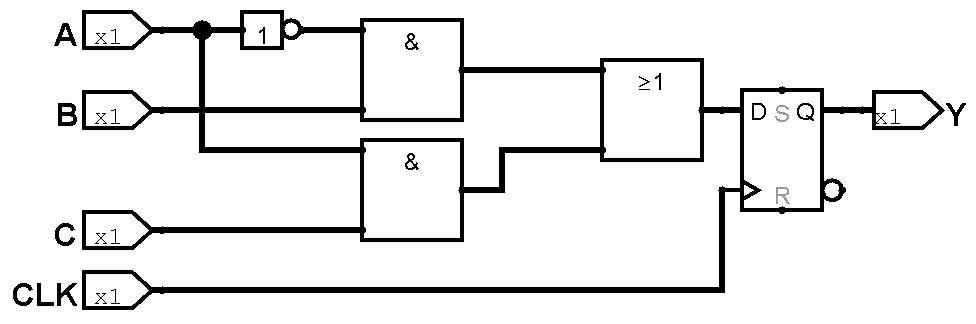
\includegraphics[scale=0.25]{fig/hazard_static_sync.png}
		\end{center}
		
		\begin{minipage}[t][\textheight][t]{0.48\textwidth}
		
		\textbf{Předpoklad:}
		
		\begin{itemize}
			\item Vstupy jsou synchronizovány na hranu \textbf{CLK} $\Rightarrow$ mění se všechny současně.
		\end{itemize}
			
		\end{minipage}
		\begin{minipage}[t][\textheight][t]{0.48\textwidth}
		
		\textbf{Výsledek:}
		
		\begin{itemize}
			\item Výsledek je zapsán s hranou \textbf{CLK} až po odeznění hazardu,
			\item zvyšujeme zpoždění získání příslušného výsledku o 1 periodu \textbf{CLK}.
		\end{itemize}
		
		\end{minipage}
	\end{frame}
	
% =====================================================================================================================
	\begin{frame}
    \frametitle{Co z toho všeho plyne pro praxi}
		
		\begin{itemize}
			\item Vždy realizujeme synchronní obvody - platí i (hlavně) v hradlových polích,
			\item výsledky kombinační logiky synchronizujeme na hranu hodin pomocí klopných obvodů (např. D KO),
			\item čtení vstupů také synchronizujeme (vzorkujeme) pomocí D KO,
			\item výsledek logiky má vždy definované zpoždění v počtu period hodinového cyklu.
		\end{itemize}
		
	\end{frame}